\documentclass{beamer}
\usetheme{tokitex}

\usepackage{tikz}
\usepackage{graphics}
\usepackage{multirow}
\usepackage{tabto}
\usepackage{xspace}
\usepackage{amsmath}
\usepackage{hyperref}
\usepackage{wrapfig}
\usepackage{mathtools}

\usepackage{tikz}
\usepackage{clrscode3e}
\usepackage{gensymb}

\usepackage[english,bahasa]{babel}
\newtranslation[to=bahasa]{Section}{Bagian}
\newtranslation[to=bahasa]{Subsection}{Subbagian}

\usepackage{listings, lstautogobble}
\usepackage{color}

\definecolor{dkgreen}{rgb}{0,0.6,0}
\definecolor{gray}{rgb}{0.5,0.5,0.5}
\definecolor{mauve}{rgb}{0.58,0,0.82}

\lstset{frame=tb,
  language=c++,
  aboveskip=0mm,
  belowskip=0mm,
  showstringspaces=false,
  columns=fullflexible,
  keepspaces=true,
  basicstyle={\small\ttfamily},
  numbers=none,
  numberstyle=\tiny\color{gray},
  keywordstyle=\color{blue},
  commentstyle=\color{dkgreen},
  stringstyle=\color{mauve},
  breaklines=true,
  breakatwhitespace=true,
  lineskip={-3pt}
}

\usepackage{caption}
\captionsetup[figure]{labelformat=empty}

\newcommand{\progTerm}[1]{\textbf{#1}}
\newcommand{\foreignTerm}[1]{\textit{#1}}
\newcommand{\newTerm}[1]{\alert{\textbf{#1}}}
\newcommand{\emp}[1]{\alert{#1}}
\newcommand{\statement}[1]{"#1"}

\newcommand{\floor}[1]{\lfloor #1 \rfloor}
\newcommand{\ceil}[1]{\lceil #1 \rceil}
\newcommand{\abs}[1]{\left\lvert#1\right\rvert}
\newcommand{\norm}[1]{\left\lVert#1\right\rVert}

% Getting tired of writing \foreignTerm all the time
\newcommand{\farray}{\foreignTerm{array}\xspace}
\newcommand{\fArray}{\foreignTerm{Array}\xspace}
\newcommand{\foverhead}{\foreignTerm{overhead}\xspace}
\newcommand{\fOverhead}{\foreignTerm{Overhead}\xspace}
\newcommand{\fsubarray}{\foreignTerm{subarray}\xspace}
\newcommand{\fSubarray}{\foreignTerm{Subarray}\xspace}
\newcommand{\fbasecase}{\foreignTerm{base case}\xspace}
\newcommand{\fBasecase}{\foreignTerm{Base case}\xspace}
\newcommand{\ftopdown}{\foreignTerm{top-down}\xspace}
\newcommand{\fTopdown}{\foreignTerm{Top-down}\xspace}
\newcommand{\fbottomup}{\foreignTerm{bottom-up}\xspace}
\newcommand{\fBottomup}{\foreignTerm{Bottom-up}\xspace}
\newcommand{\fpruning}{\foreignTerm{pruning}\xspace}
\newcommand{\fPruning}{\foreignTerm{Pruning}\xspace}

\newcommand{\fgraph}{\foreignTerm{graph}\xspace}
\newcommand{\fGraph}{\foreignTerm{Graph}\xspace}
\newcommand{\froot}{\foreignTerm{root}\xspace}
\newcommand{\fRoot}{\foreignTerm{Root}\xspace}
\newcommand{\fnode}{\foreignTerm{node}\xspace}
\newcommand{\fNode}{\foreignTerm{Node}\xspace}
\newcommand{\fedge}{\foreignTerm{edge}\xspace}
\newcommand{\fEdge}{\foreignTerm{Edge}\xspace}
\newcommand{\fcycle}{\foreignTerm{cycle}\xspace}
\newcommand{\fCycle}{\foreignTerm{Cycle}\xspace}
\newcommand{\fdegree}{\foreignTerm{degree}\xspace}
\newcommand{\fDegree}{\foreignTerm{Degree}\xspace}
\newcommand{\fadjacencylist}{\foreignTerm{adjacency list}\xspace}
\newcommand{\fAdjacencylist}{\foreignTerm{Adjacency list}\xspace}
\newcommand{\fadjacencymatrix}{\foreignTerm{adjacency matrix}\xspace}
\newcommand{\fAdjacencymatrix}{\foreignTerm{Adjacency matrix}\xspace}
\newcommand{\fedgelist}{\foreignTerm{edge list}\xspace}
\newcommand{\fEdgelist}{\foreignTerm{Edge list}\xspace}
\newcommand{\flist}{\foreignTerm{list}\xspace}
\newcommand{\fList}{\foreignTerm{List}\xspace}
\newcommand{\fgraphtraversal}{\foreignTerm{graph traversal}\xspace}
\newcommand{\fGraphtraversal}{\foreignTerm{Graph traversal}\xspace}
\newcommand{\ftree}{\foreignTerm{tree}\xspace}
\newcommand{\fTree}{\foreignTerm{Tree}\xspace}
\newcommand{\fsubtree}{\foreignTerm{subtree}\xspace}
\newcommand{\fSubtree}{\foreignTerm{Subtree}\xspace}
\newcommand{\fparent}{\foreignTerm{parent}\xspace}
\newcommand{\fParent}{\foreignTerm{Parent}\xspace}
\newcommand{\fsibling}{\foreignTerm{sibling}\xspace}
\newcommand{\fSibling}{\foreignTerm{Sibling}\xspace}
\newcommand{\fpath}{\foreignTerm{path}\xspace}
\newcommand{\fPath}{\foreignTerm{Path}\xspace}
\newcommand{\fconnectedcomponent}{\foreignTerm{connected component}\xspace}
\newcommand{\fConnectedcomponent}{\foreignTerm{Connected component}\xspace}
\newcommand{\fbridge}{\foreignTerm{bridge}\xspace}
\newcommand{\fBridge}{\foreignTerm{Bridge}\xspace}
\newcommand{\farticulationpoint}{\foreignTerm{articulation point}\xspace}
\newcommand{\fArticulationpoint}{\foreignTerm{Articulation point}\xspace}
\newcommand{\ftreeedge}{\foreignTerm{tree edge}\xspace}
\newcommand{\fTreeedge}{\foreignTerm{Tree edge}\xspace}
\newcommand{\fbackedge}{\foreignTerm{back edge}\xspace}
\newcommand{\fBackedge}{\foreignTerm{Back edge}\xspace}
\newcommand{\fforwardedge}{\foreignTerm{forward edge}\xspace}
\newcommand{\fForwardedge}{\foreignTerm{Forward edge}\xspace}
\newcommand{\fcrossedge}{\foreignTerm{cross edge}\xspace}
\newcommand{\fCrossedge}{\foreignTerm{Cross edge}\xspace}
\newcommand{\fdiscoverytime}{\foreignTerm{discovery time}\xspace}
\newcommand{\fDiscoverytime}{\foreignTerm{Discovery time}\xspace}
\newcommand{\flowlink}{\foreignTerm{low link}\xspace}
\newcommand{\fLowlink}{\foreignTerm{Low link}\xspace}
\newcommand{\fstack}{\foreignTerm{stack}\xspace}
\newcommand{\fStack}{\foreignTerm{Stack}\xspace}
\newcommand{\for}{\foreignTerm{or}\xspace}
\newcommand{\fOr}{\foreignTerm{Or}\xspace}
\newcommand{\fand}{\foreignTerm{and}\xspace}
\newcommand{\fAnd}{\foreignTerm{And}\xspace}
\newcommand{\fcentroid}{\foreignTerm{centroid}\xspace}
\newcommand{\fCentroid}{\foreignTerm{Centroid}\xspace}

\newcommand{\fDivideAndConquer}{\foreignTerm{Divide and conquer}\xspace}
\newcommand{\fdivideAndConquer}{\foreignTerm{divide and conquer}\xspace}
\newcommand{\fMergeSort}{\foreignTerm{Merge sort}\xspace}
\newcommand{\fmergeSort}{\foreignTerm{merge sort}\xspace}
\newcommand{\fQuickSort}{\foreignTerm{Quicksort}\xspace}
\newcommand{\fquickSort}{\foreignTerm{quicksort}\xspace}
\newcommand{\fpivot}{\foreignTerm{pivot}\xspace}
\newcommand{\fPivot}{\foreignTerm{Pivot}\xspace}
\newcommand{\fbruteForce}{\foreignTerm{brute force}\xspace}
\newcommand{\fBruteForce}{\foreignTerm{Brute force}\xspace}
\newcommand{\fCompleteSearch}{\foreignTerm{complete search}\xspace}
\newcommand{\fExhaustiveSearch}{\foreignTerm{exhaustive search}\xspace}
\newcommand{\fbinarySearch}{\foreignTerm{binary search}\xspace}
\newcommand{\fBinarySearch}{\foreignTerm{Binary search}\xspace}
\newcommand{\fternarySearch}{\foreignTerm{ternary search}\xspace}
\newcommand{\fTernarySearch}{\foreignTerm{Ternary search}\xspace}
\newcommand{\funimodal}{\foreignTerm{unimodal}\xspace}
\newcommand{\fUnimodal}{\foreignTerm{Unimodal}\xspace}
\newcommand{\fGreedy}{\foreignTerm{Greedy}\xspace}
\newcommand{\fgreedy}{\foreignTerm{greedy}\xspace}
\newcommand{\fgreedyChoice}{\foreignTerm{greedy choice}\xspace}
\newcommand{\fGreedyChoice}{\foreignTerm{Greedy choice}\xspace}

\newcommand{\fdp}{\foreignTerm{dynamic programming}\xspace}
\newcommand{\fDp}{\foreignTerm{Dynamic programming}\xspace}
\newcommand{\fbitmask}{\foreignTerm{bitmask}\xspace}
\newcommand{\fBitmask}{\foreignTerm{Bitmask}\xspace}
\newcommand{\fstate}{\foreignTerm{state}\xspace}
\newcommand{\fState}{\foreignTerm{State}\xspace}
\newcommand{\fsubmask}{\foreignTerm{submask}\xspace}
\newcommand{\fSubmask}{\foreignTerm{Submask}\xspace}

\newcommand{\pheap}{\foreignTerm{heap}\xspace}
\newcommand{\pHeap}{\foreignTerm{Heap}\xspace}
\newcommand{\pBinaryHeap}{\foreignTerm{Binary Heap}\xspace}
\newcommand{\pbinaryHeap}{\foreignTerm{binary heap}\xspace}
\newcommand{\pHeapsort}{\foreignTerm{Heapsort}\xspace}
\newcommand{\pheapsort}{\foreignTerm{heapsort}\xspace}
\newcommand{\pdjs}{\foreignTerm{disjoint set}\xspace}
\newcommand{\pDjs}{\foreignTerm{Disjoint set}\xspace}

\newcommand{\fdotProduct}{\foreignTerm{dot product}\xspace}
\newcommand{\fDotProduct}{\foreignTerm{Dot product}\xspace}
\newcommand{\fcrossProduct}{\foreignTerm{cross product}\xspace}
\newcommand{\fCrossProduct}{\foreignTerm{Cross product}\xspace}
\newcommand{\fconvexHull}{\foreignTerm{convex hull}\xspace}
\newcommand{\fConvexHull}{\foreignTerm{Convex hull}\xspace}
\newcommand{\fgrahamScan}{\foreignTerm{graham scan}\xspace}
\newcommand{\fGrahamScan}{\foreignTerm{Graham scan}\xspace}
\newcommand{\flineSweep}{\foreignTerm{line sweep}\xspace}
\newcommand{\fLineSweep}{\foreignTerm{Line sweep}\xspace}

\newcommand{\fset}{\foreignTerm{set}\xspace}
\newcommand{\fSet}{\foreignTerm{Set}\xspace}
\newcommand{\fprefixSum}{\foreignTerm{prefix sum}\xspace}
\newcommand{\fPrefixSum}{\foreignTerm{Prefix sum}\xspace}
\newcommand{\ffenwickTree}{\foreignTerm{fenwick tree}\xspace}
\newcommand{\fFenwickTree}{\foreignTerm{Fenwick tree}\xspace}
\newcommand{\frangeSumQuery}{\foreignTerm{range sum query}\xspace}
\newcommand{\fRangeSumQuery}{\foreignTerm{Range sum query}\xspace}
\newcommand{\fquery}{\foreignTerm{query}\xspace}
\newcommand{\fQuery}{\foreignTerm{Query}\xspace}
\newcommand{\fsegmentTree}{\foreignTerm{segment tree}\xspace}
\newcommand{\fSegmentTree}{\foreignTerm{Segment tree}\xspace}
\newcommand{\fbinaryTree}{\foreignTerm{binary tree}\xspace}
\newcommand{\fBinaryTree}{\foreignTerm{Binary tree}\xspace}
\newcommand{\flazyPropagation}{\foreignTerm{lazy propagation}\xspace}
\newcommand{\fLazyPropagation}{\foreignTerm{Lazy propagation}\xspace}
\newcommand{\fsparseTable}{\foreignTerm{sparse table}\xspace}
\newcommand{\fSparseTable}{\foreignTerm{Sparse table}\xspace}

\newcommand{\ftrail}{\foreignTerm{trail}\xspace}
\newcommand{\fTrail}{\foreignTerm{Trail}\xspace}
\newcommand{\feulerTour}{\foreignTerm{euler tour}\xspace}
\newcommand{\fEulerTour}{\foreignTerm{Euler tour}\xspace}
\newcommand{\feulerTourTree}{\foreignTerm{euler tour tree}\xspace}
\newcommand{\fEulerTourTree}{\foreignTerm{Euler tour tree}\xspace}

\newcommand{\fmaxflow}{\foreignTerm{maximum flow}\xspace}
\newcommand{\fMaxflow}{\foreignTerm{Maximum flow}\xspace}
\newcommand{\fmincut}{\foreignTerm{minimum cut}\xspace}
\newcommand{\fMincut}{\foreignTerm{Minimum cut}\xspace}
\newcommand{\fflow}{\foreignTerm{flow}\xspace}
\newcommand{\fFlow}{\foreignTerm{Flow}\xspace}
\newcommand{\fsource}{\foreignTerm{source}\xspace}
\newcommand{\fSource}{\foreignTerm{Source}\xspace}
\newcommand{\fsink}{\foreignTerm{sink}\xspace}
\newcommand{\fSink}{\foreignTerm{Sink}\xspace}
\newcommand{\fbackEdge}{\foreignTerm{back-edge}\xspace}
\newcommand{\fBackEdge}{\foreignTerm{Back-edge}\xspace}
\newcommand{\fresidualCapacity}{\foreignTerm{residual capacity}\xspace}
\newcommand{\fResidualCapacity}{\foreignTerm{Residual capacity}\xspace}
\newcommand{\fbottleneck}{\foreignTerm{bottleneck}\xspace}
\newcommand{\fBottleneck}{\foreignTerm{Bottleneck}\xspace}
\newcommand{\faugmentingPath}{\foreignTerm{augmenting path}\xspace}
\newcommand{\fAugmentingPath}{\foreignTerm{Augmenting path}\xspace}


\title{Geometri Komputasional}
\author{Tim Olimpiade Komputer Indonesia}
\date{}

\begin{document}

\begin{frame}
\titlepage
\end{frame}

\begin{frame}
\frametitle{Pendahuluan}
Melalui dokumen ini, kalian akan:
\begin{itemize}
  \item Memahami konsep vektor
  \item Memahami konsep poligon
  \item Memahami konsep convex hull
  \item Memahami konsep line sweep
\end{itemize}
\end{frame}

\begin{frame}
\frametitle{Vektor}
\begin{itemize}
  \item \newTerm{Vektor} adalah objek matematika yang memiliki besaran dan arah.
  \begin{itemize}
    \item Sebagai contoh, "10 langkah ke utara" pada instruksi "berjalan 10 langkah ke utara" adalah sebuah vektor, karena "10 langkah" merupakan besaran dan "ke utara" merupakan arah. 
  \end{itemize}
  \item Dua vektor dibandingkan dengan besaran dan arahnya.
  \begin{itemize}
    \item Sebagai contoh, "10 langkah ke utara" pada instruksi "berjalan 10 langkah ke utara dari titik A" dan "berjalan 10 langkah ke utara dari titik B" adalah dua vektor yang sama.
    \item Namun, "10 langkah ke utara" dan "10 langkah ke selatan" adalah dua vektor yang berbeda.
  \end{itemize}
\end{itemize}
\end{frame}

\begin{frame}
\frametitle{Notasi Vektor}
\begin{itemize}
  \item Sebuah vektor biasanya dinotasikan dengan tanda panah di atas variabelnya (contoh: $\overrightarrow{v}$).
  \item Besaran vektor $\overrightarrow{v}$ dinotasikan dengan $\norm{\overrightarrow{v}}$.
  \item Pada ruang Euklides $n$ dimensi, sebuah vektor $\overrightarrow{v}$ biasanya direpresentasikan dalam $n$ bilangan: $(v_1, v_2, \dots, v_n)$, dengan $v_i$ adalah besaran vektor pada arah dimensi ke-$i$.
  \begin{itemize}
    \item Menggunakan teorema Pythagoras, $\norm{\overrightarrow{v}} = \sqrt{\sum_{i=1}^{n} v_i}$.
    \item Pada dokumen ini, kita akan mengasumsikan seluruh vektor berada pada ruang Euklides $n$ dimensi.
  \end{itemize}
\end{itemize}
\end{frame}

\begin{frame}
\frametitle{Operasi Vektor}
\begin{itemize}
  \item Penjumlahan dua vektor dinotasikan dengan $\overrightarrow{v} + \overrightarrow{w}$ dan dapat dihitung dengan menjumlahkan besaran pada setiap dimensinya.
  \item Negasi vektor dinotasikan dengan $-\overrightarrow{v}$ dan dapat dihitung dengan menegasikan besaran pada setiap dimensinya.
  \item Perkalian vektor dan skalar dinotasikan dengan $k\overrightarrow{v}$ dan dapat dihitung dengan mengkalikan besaran pada setiap dimensinya dengan $k$.
  \item \newTerm{Dot product} dua vektor adalah sebuah skalar yang dinotasikan dengan $\overrightarrow{v} \cdot \overrightarrow{w}$ dan dapat dihitung dengan menjumlahkan perkalian besaran pada setiap dimensinya.
  \item \newTerm{Cross product} dua vektor $3$ dimensi adalah sebuah vektor $3$ dimensi yang dinotasikan dengan $\overrightarrow{v} \times \overrightarrow{w} = (v_2w_3 - v_3w_2, v_3w_1 - v_1w_3, v_1w_2 - v_2w_1)$.
\end{itemize}
\end{frame}

\begin{frame}
\frametitle{Operasi Vektor: Contoh}
Sebagai contoh, jika $\overrightarrow{AB} = (1, 1), \overrightarrow{AC} = (2, 0)$.
\begin{itemize}
  \item $\overrightarrow{AC} + \overrightarrow{AB} = (2 + 1, 0 + 1) = (3, 1)$
  \item $-\overrightarrow{AB} = (-1, -1)$
  \item $\overrightarrow{AC} - \overrightarrow{AB} = (2 - 1, 0 - 1) = (1, -1)$
  \item $4\overrightarrow{AB} = (4 \times 1, 4 \times 1) = (4, 4)$
  \item $\overrightarrow{AB} \cdot \overrightarrow{AC} = 1 \times 2 + 1 \times 0 = 2$
\end{itemize}
\begin{center}
  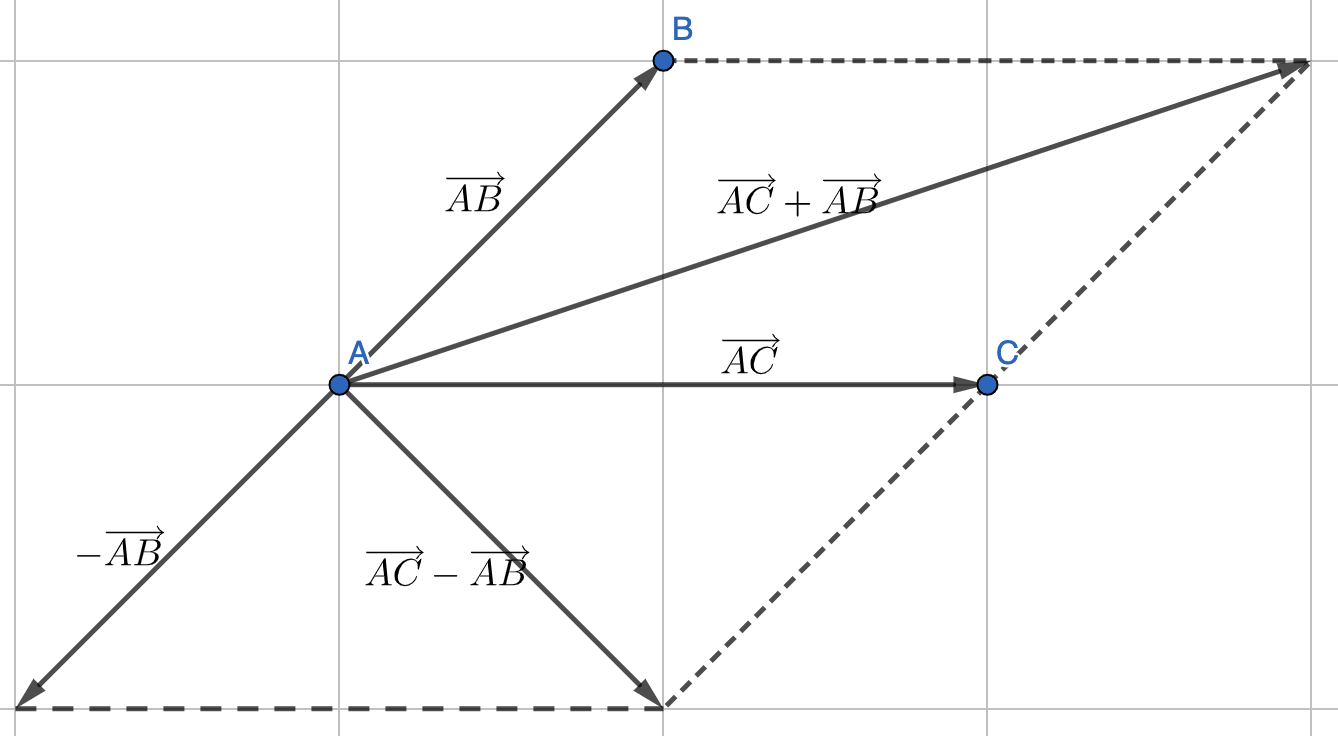
\includegraphics[width=6cm]{asset/vector-operations.png}
\end{center}
\end{frame}

\begin{frame}
\frametitle{Penggunaan Cross Product}
\begin{itemize}
  \item Pada bidang 2 dimensi, jika kita memiliki tiga titik $O = (x_O, y_O), A = (x_A, y_A), B = (x_B, y_B)$, kita dapat menghitung apakah sudut yang dibentuk oleh ketiga titik tersebut positif menggunakan \fcrossProduct.
  \begin{itemize}
    \item Hitung besaran pada arah dimensi ketiga dari vektor $\overrightarrow{OA}$ dan $\overrightarrow{OB}$. Untuk lebih mudahnya, anggap nilai $P$ adalah $(x_A - x_O)(y_B - y_O) - (y_A - y_O)(x_B - x_O)$.
    \item Jika $P > 0$, maka sudut $OAB$ berlawanan arah jarum jam. Dengan kata lain, $B$ berada di kiri garis $OA$.
    \item Jika $P < 0$, maka sudut $OAB$ searah jarum jam. Dengan kata lain, $B$ berada di kanan garis $OA$.
    \item Jika $P = 0$, maka titik $O$, $A$, dan $B$ berada pada garis yang sama. 
  \end{itemize}
\end{itemize}
\end{frame}

\begin{frame}
\frametitle{Poligon}
\begin{itemize}
  \item \newTerm{Poligon} adalah bentuk datar yang terdiri dari titik (disebut titik sudut) serta garis yang menghubungkan titik sudut dan membentuk lintasan tertutup.
  \item \newTerm{Poligon cembung} (\foreignTerm{convex polygon}\xspace) adalah poligon dengan besar seluruh sudut dalam kurang dari $180\degree$.
  \begin{itemize}

    \item Dengan kata lain, tidak terdapat segmen garis di antara dua titik pada batas poligon yang keluar dari poligon.
  \end{itemize}
  \item \newTerm{Poligon cekung} (\foreignTerm{concave polygon}\xspace) adalah poligon dengan besar setidaknya satu sudut dalam tidak kurang dari $180\degree$.
\end{itemize}
\begin{center}
  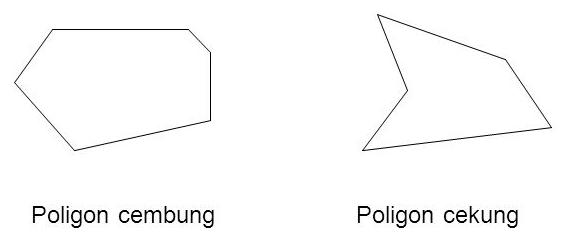
\includegraphics[width=6cm]{asset/polygon-convex-concave.png}
\end{center}
\end{frame}

\begin{frame}
\frametitle{Luas Poligon}
\begin{itemize}
  \item \newTerm{Shoelace formula} adalah rumus yang dapat digunakan untuk menghitung luas poligon.
  \item Poligon dengan titik sudut $(x_1, y_1), (x_2, y_2), \dots, (x_n, y_n)$ memiliki luas
  \[\frac{1}{2}\abs{\sum_{i=1}^n x_iy_{i+1} - \sum_{i=1}^n x_{i+1}y_i}\]
  \[= \frac{1}{2}\abs{x_1y_2 + x2y_3 + \dots + x_ny_{n+1} - x_2y_1 - x_3y_2 - \dots - x_{n+1}y_n}\]
  dengan $(x_{n+1}, y_{n+1}) = (x_1, y_1)$.
\end{itemize}
\end{frame}

\begin{frame}
\frametitle{Lokasi Titik pada Poligon}
\begin{itemize}
  \item Untuk poligon cembung, jika terdapat titik $P = (x, y)$, maka kita dapat menentukan lokasi titik berada pada di dalam atau di luar poligon menggunakan \fcrossProduct.
  \begin{itemize}
    \item Untuk semua titik bersebelahan $A$ dan $B$ pada poligon, hitung arah dari sudut $PAB$.
    \item Jika semua sudut $PAB$ berlawanan arah jarum jam atau berada pada garis yang sama, maka titik berada di dalam poligon.
    \item Jika semua sudut $PAB$ searah arah jarum jam atau berada pada garis yang sama, maka titik berada di dalam poligon.
    \item Jika terdapat sudut $PAB$ yang searah dan berlawanan arah jarum jam, maka titik berada di luar poligon.
  \end{itemize}
\end{itemize}
\end{frame}

\begin{frame}
\frametitle{Convex Hull}
\begin{itemize}
  \item Pada $2$ dimensi, \newTerm{convex hull} dari himpunan titik adalah poligon cembung terkecil yang mencakup seluruh titik tersebut.
  \item \fConvexHull dapat dibayangkan seperti karet yang cukup besar dan terdapat paku pada setiap titik, kemudian karet tersebut dilepaskan. Bentuk akhir dari karet membentuk \fconvexHull.
  \item Pada pembahasan ini, kita ingin mencari titik-titik yang membentuk \fconvexHull (himpunan titik-titik yang disentuh oleh karet).
\end{itemize}
\begin{center}
  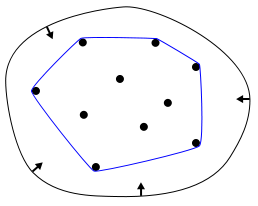
\includegraphics[width=4cm]{asset/convex-hull.png}
\end{center}
\end{frame}

\begin{frame}
\frametitle{Graham Scan}
\begin{itemize}
  \item Salah satu metode untuk mencari \fconvexHull adalah menggunakan algoritme \newTerm{Graham scan}.
  \item Algoritme ini mengambil titik yang berada di paling bawah (koordinat y terkecil) sebagai \fpivot dan bagian dari \fconvexHull.
  \item Lakukan pengurutan titik-titik lainnya berdasarkan sudut polar terhadap \fpivot. Dengan kata lain, titik $A$ lebih kecil dari titik $B$ jika titik $B$ berada di kiri garis $OA$ dengan titik $O$ adalah \fpivot.
\end{itemize}
\end{frame}

\begin{frame}
\frametitle{Graham Scan (lanj.)}
\begin{itemize}
  \item Kemudian, algoritme ini mencoba untuk memasukkan titik-titik lainnya satu per satu ke dalam \fconvexHull, diurutkan dari yang paling kecil.
  \begin{itemize}
    \item Misalkan titik $R$ adalah titik yang sekarang sedang diperhatikan, $Q$ adalah titik terakhir pada \fconvexHull sementara, dan titik $P$ adalah titik sebelum titik $Q$ pada \fconvexHull sementara.
    \item Jika titik $R$ berada di kanan garis $PQ$, maka dapat dipastikan titik $Q$ tidak berada di dalam \fconvexHull. Karenanya, kita dapat mengeluarkan titik $Q$ pada \fconvexHull sementara.
    \item Perbaharui titik $P$ dan titik $Q$ menggunakan definisi di atas.
    \item Kita dapat melakukan hal yang sama sampai titik $R$ berada di kiri garis $PQ$, atau terdapat hanya satu titik pada \fconvexHull.
  \end{itemize}
  \item Kompleksitas algoritme ini adalah $O(N \log N)$, dengan $N$ adalah banyaknya titik.
\end{itemize}
\end{frame}

\begin{frame}[fragile]
\frametitle{Graham Scan (lanj.)}
\begin{lstlisting}
typedef pair<int, int> Point;
#define x first
#define y second

bool turn_right(Point o, Point p, Point q) {
  return (p.x - o.x) * (q.y - o.y) < (p.y - o.y) * (q.x - o.x);
}

vector<Point> convex_hull(vector<Point> P) {
  // Letakan pivot di P[0].
  for (int i = 1; i < P.size(); ++i) {
    if (P[i].y < P[0].y) {
      swap(P[0], P[i]);
    }
  }

  sort(P.begin() + 1, P.end(), [&] (Point p, Point q) {
    return turn_right(P[0], q, p);
  });

...
\end{lstlisting}
\end{frame}

\begin{frame}[fragile]
\frametitle{Graham Scan (lanj.)}
\begin{lstlisting}
  vector<Point> convex_hull = {P[0]};

  for (int i = 1; i < P.size(); ++i) {
    while (convex_hull.size() > 1) {
      Point p = convex_hull[convex_hull.size() - 2];
      Point q = convex_hull[convex_hull.size() - 1];
      if (turn_right(p, q, P[i])) {
        break;
      }
    }
    convex_hull.push_back(P[i]);
  }

  return convex_hull;
}
\end{lstlisting}
\end{frame}

\begin{frame}
\frametitle{Algoritme Convex Hull lain}
\begin{itemize}
  \item Sebagai tambahan informasi, selain algoritme \fGrahamScan terdapat beberapa algoritme lain yang cukup umum:
  \begin{itemize}
    \item Algoritme \newTerm{Gift wrapping} (sering juga disebut \newTerm{Jarvis march}) mencari \fconvexHull dalam waktu $O(NH)$, dengan $H$ adalah banyaknya titik pada \fconvexHull.
    \item Algoritme \newTerm{Monotone chain} (sering juga disebut \newTerm{Andrew's algorithm}) mencari \fconvexHull dalam waktu $O(N \log N)$.
  \end{itemize}
  \item Kita tidak akan membahas algoritme tersebut pada diskusi ini.
\end{itemize}
\end{frame}

\begin{frame}[fragile]
\frametitle{Line Sweep}
\begin{itemize}
  \item Algoritme \newTerm{line sweep} menyapu (\foreignTerm{sweep}\xspace) garis untuk menyelesaikan beberapa soal pada bidang $2$ dimensi.
  \item Contoh soal: diberikan himpunan $A$ yang berisi $N$ segmen garis yang sejajar dengan sumbu $x$ dan himpunan $B$ yang berisi $N$ segmen garis yang sejajar dengan sumbu $y$. Tentukan apakah terdapat segmen garis pada himpunan $A$ yang berpotongan dengan segmen garis pada himpuan $B$.
  \item Soal ini dapat diselesaikan dengan menyimpan koordinat x dari setiap \newTerm{peristiwa}, yang merupakan salah satu dari:
  \begin{itemize}
    \item ujung kiri dari segmen garis pada himpunan $A$,
    \item ujung kanan dari segmen garis pada himpuan $A$,
    \item segmen garis pada himpunan $B$.
  \end{itemize}
\end{itemize}
\end{frame}

\begin{frame}[fragile]
\frametitle{Line Sweep (lanj.)}
\begin{itemize}
  \item Peristiwa diproses satu per satu dengan urutan koordinat $x$ menaik, sehingga seperti penyapuan garis. Kita juga membutuhkan sebuah struktur data $D$.
  \begin{itemize}
    \item Jika peristiwa merupakan ujung kiri dari segmen garis pada himpunan $A$, maka tambahkan koordinat y garis tersebut pada $D$.
    \item Jika peristiwa merupakan ujung kanan dari segmen garis pada himpunan $A$, maka hapus koordinat y garis tersebut pada $D$.
    \item Jika peristiwa merupakan segmen garis pada himpunan $B$, maka periksa apakah terdapat bilangan pada $D$ yang berada di antara $y_{\min}$ dan $y_{\max}$.
    \begin{itemize}
      \item Jika ada, maka segmen garis ini berpotongan dengan segmen garis pada himpunan $A$.
    \end{itemize}
  \end{itemize}
  \item Kita dapat menggunakan struktur data C++ \textbf{set} (akan dibahas pada materi berikutnya) agar seluruh penambahan dan pengecekan pada $D$ membutuhkan waktu $O(\log N)$.
  \begin{itemize}
    \item Sehingga, total kompleksitas waktu solusi ini adalah $O(N \log N)$.
  \end{itemize}
\end{itemize}
\end{frame}

\end{document}
